\documentclass{article}
\usepackage{amsfonts, amsmath, amssymb, amsthm} % Math notations imported
\usepackage{enumitem}
\usepackage{graphicx}
\usepackage{setspace}
\usepackage{indentfirst}
\usepackage[margin=1in]{geometry}
\graphicspath{{./images/}} % Path to images

% \begin{figure}[htb!]
%      \centering
%      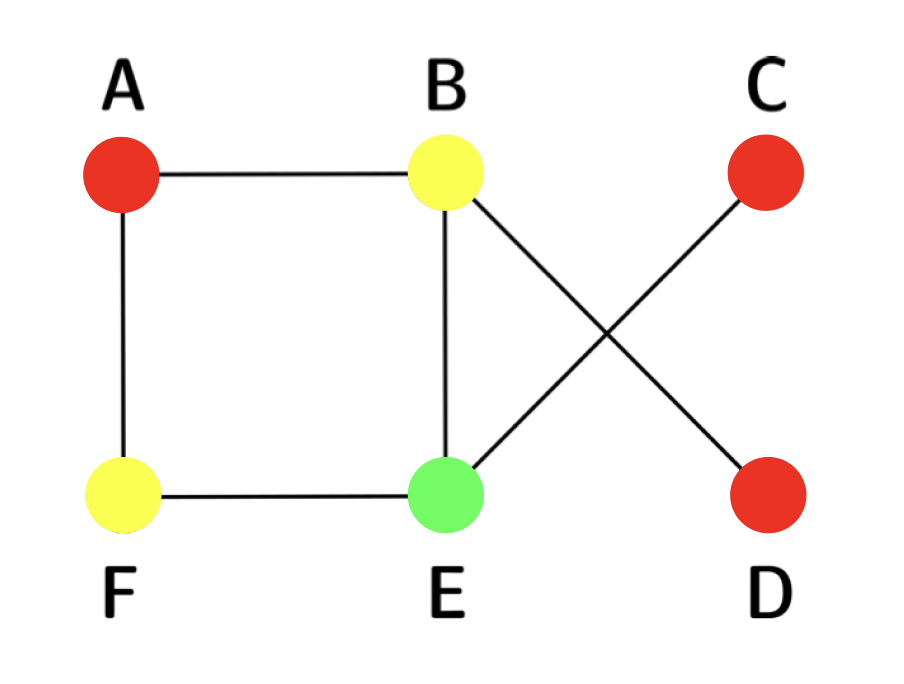
\includegraphics[scale=0.5]{coloring.png}
%      \caption{Coloring of the graph.}
% \end{figure}

% \begin{figure}[htb]
%     \qquad
%     \begin{minipage}{.4\textwidth}
%         \centering
%         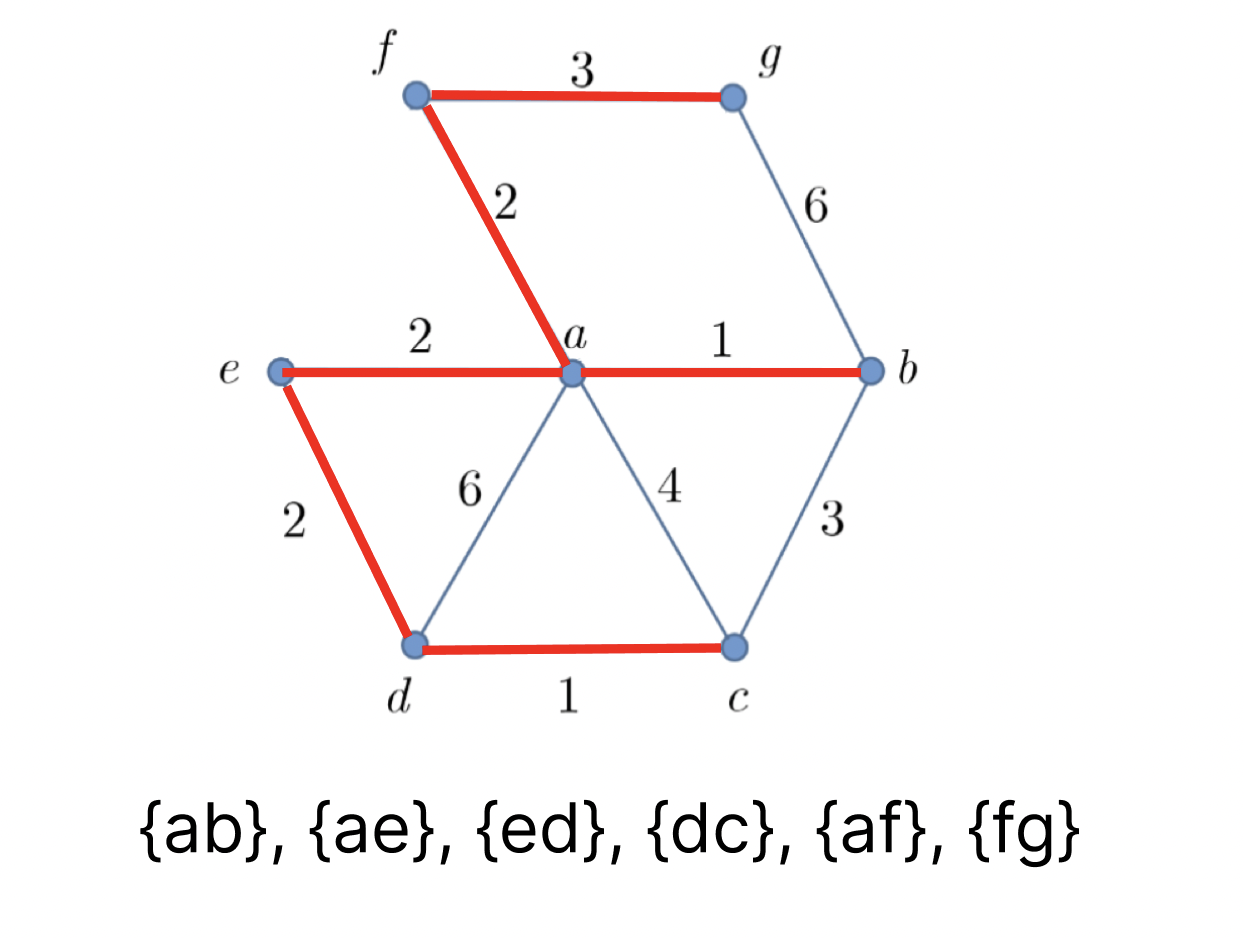
\includegraphics[scale=0.35]{prims.png}
%         \caption{}
%     \end{minipage}    
%     \qquad
%     \begin{minipage}{.4\textwidth}
%         \centering
%         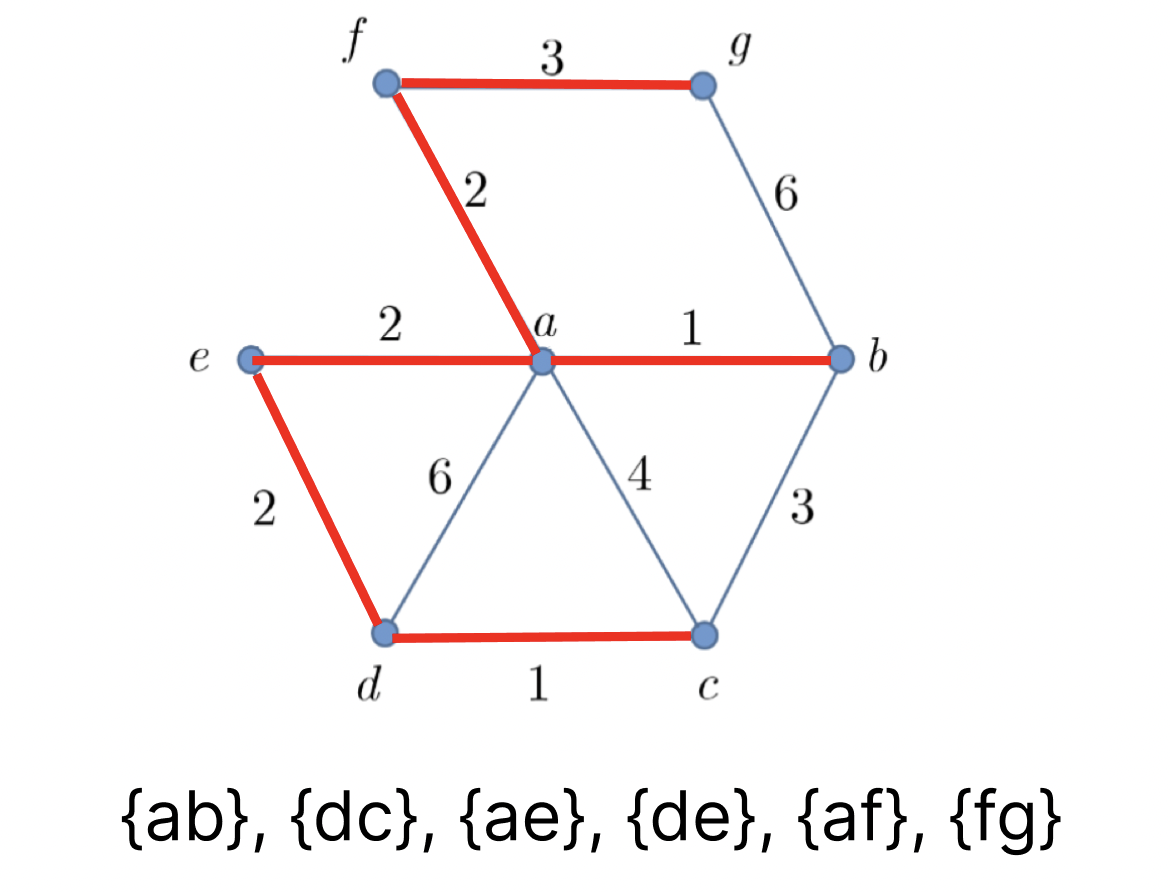
\includegraphics[scale=0.35]{kruskal.png}
%         \caption{}
%     \end{minipage}        
% \end{figure} 

\newtheorem{thm}{Theorem}
\newtheorem{proposition}[thm]{Proposition}
\newtheorem{cor}[thm]{Corollary}

% title information
\title{Math 110 HW3}
\author{Neo Lee}
\date{09/16/2023}

\setstretch{1.15}
% main content
\begin{document} 

% placing title information; comment out if using fancyhdr
\maketitle 

\subsection*{Problem 1}
Let $U:=\{p\in\mathcal{P}_2(\mathbb{R}):\int_{-1}^{1}(xp''(x)+p'(x))dx=0\}.$
\begin{description}
    \item{(a)} Find a basis for $U$. 
    \begin{proof}[Solution]
        Let's rewrite $U$ in a simpler form. We know every $p\in\mathcal{P}_2(\mathbb{R})$ can be 
        written as $p(x)=ax^2+bx+c$. Then we have
        \begin{align*}
            p''(x) & = 2a \\
            p'(x) & = 2ax + b.
        \end{align*}
        Now, 
        \begin{align*}
            \int_{-1}^{1}(xp''(x)+p'(x))dx & = 0 \\
            \int_{-1}^{1}(x(2a)+2ax+b)dx & = 0 \\
            \int_{-1}^{1}(2ax+2ax+b)dx & = 0 \\
            \int_{-1}^{1}(4ax)dx + \int_{-1}^{1}b dx & = 0 \\
            4a\int_{-1}^{1}xdx + b\int_{-1}^{1}dx & = 0 \\
            4a\left[\frac{x^2}{2}\right]_{-1}^{1} + b\left[x\right]_{-1}^{1} & = 0 \\
            4a \left(\frac{1}{2}-\frac{1}{2}\right)+ b(1-(-1)) & = 0 \\
            2b & = 0 \\
            b & = 0.
        \end{align*}

        Therefore, $U=\{p\in\mathcal{P}_2(\mathbb{R}):p(x)=ax^2+c\} = \{ax^2+c:a,c\in\mathbb{R}\}$. 
        Now, we can see clearly that 
        the basis of $U$ is $\{x^2, 1\}$ as every $p\in U$ can be written as $p(x)=ax^2+c$ for $a,c
        \in \mathbb{R}$ and $\{x^2, 1\}$ are linearly independent.
    \end{proof}

    \newpage
    \item{(b)} Extend your basis in part (a) to a basis of ${\mathcal P}_3(\mathbb{R})$.
    \begin{proof}[Solution]
        We can do this by appending the standard basis of ${\mathcal P}_3(\mathbb{R})$ to the basis 
        of $U$ in part (a), then remove all the dependent vectors. 

        After appending the basis, we get $\{x^2, 1, x^3, x^2, x, 1\}$. Now, we can remove the 
        dependent vectors, which are very obvious because they are the same. Therefore, we are left 
        with $\{x^3, x^2, x, 1\}$, which are independet and span the whole ${\mathcal P}_3(\mathbb{R})$.
    \end{proof}

    \item{(c)} Find a subspace $W$ of ${\mathcal P}_3(\mathbb{R})$ such that 
    ${\mathcal P}_3(\mathbb{R}) = U \oplus W$.
    \begin{proof}[Solution]
        Define $W:=span\{x, x^3\}$. We can see that $W$ is a subspace of ${\mathcal P}_3(\mathbb{R})$
        obviously. 

        Now we check that it is indeed a direct sum by checking their intersection. We know that 
        for $u\in U$, $u(x)=ax^2+c$ for $a,c\in\mathbb{R}$. For $w\in W$, $w(x)=bx^3+dx$ for $b,d 
        \in \mathbb{R}$. Now if $u = w$, 
        \begin{align*}
            ax^2+c & = bx^3+dx \\ 
            -bx^3+ax^2+c-dx & = 0.
        \end{align*}

        And we know that $x^3, x^2, x, 1$ are linearly independent. Therefore, $a=b=c=d=0$, and 
        $u=w=0$. Therefore, $U\cap W = \{0\}$, and $U\oplus W = {\mathcal P}_3
        (\mathbb{R})$.
    \end{proof}
\end{description}

\newpage
\subsection*{Problem 2}
Suppose $v_1, \ldots, v_m$ are linearly independent in $V$ and $w_0\in V$.  
Prove that $$ \dim span (v_1 - w_0, v_2 - w_0, \dots, v_m - w_0) \ge m-1.$$
\begin{proof}[Proof 1]
    Define $U:=span (v_1 - w_0, v_2 - w_0, \dots, v_m - w_0)$ and $W:= span(w_0)$. Now we know 
    $U+W=span(v_1,\dots, v_m, w_0)$. 
    To show this, we look at the linear combination of any $u\in U, w\in W$,
    \begin{align*}
        a_1(v_1-w_0) + \dots + a_m(v_m-w_0) + b_1w_0 & = 
        a_1v_1 + \dots + a_mv_m + (b_1-a_1-\dots -a_m)\cdot w_0 \\
        & = a_1v_1 + \dots + a_mv_m + c_0w_0.
    \end{align*}
    Also, notice $\dim span(v_1, \dots, v_m, w_0) \ge m$ since $v_1, \dots, v_m$ are linearly 
    independent. Therefore, $\dim (U+W) \ge m$.

    Now, apply the inclusion-exclusion formula, we have 
    \begin{align*}
        \dim (U+W) & = \dim (U) + \dim (W) - \dim (U\cap W) \\
        \dim(U) & = \dim (U+W) + \dim (U\cap W) - \dim (W) \\
        \dim(U) & \ge m + \dim (U\cap W) - 1 \\
        \dim(U) & \ge m - 1.
    \end{align*}
\end{proof}
\bigbreak
\begin{proof}[Proof 2]
    To simplify the notations, denote $U:=span (v_1 - w_0, v_2 - w_0, \dots, v_m - w_0) 
    = span(u_1, u_2, \dots, u_m)$ and $U' = span(u_1-u_1, u_2-u_1, u_3-u_1, \dots, u_m-u_1) = 
    span(0, v_2-v_1, v_3-v_1,\dots, v_m-v_1)$ [the 0 is trivial and can be removed].
    
    Now we want to show that $U'$ is a subspace of $U$, and $\dim (U')=m-1$. From that we can say 
    $\dim (U) \ge \dim (U') = m-1$ because a vector space cannot have a dimension smaller than its subspace.

    \bigbreak
    \underline{$U' \subseteq U$:} For arbitrary $u'\in U'$,
    \begin{align*}
        u' & = a_2(v_2-v_1) + \dots + a_m(v_m-v_1) \\
        & = a_2(u_2-u_1) + \dots + a_m(u_m-u_1) \\
        & = a_2u_2 + \dots + a_mu_m - (a_2+\dots+a_m)u_1,
    \end{align*}
    which is a linear combination of $(u_1, \dots, u_m)$. Therefore, $u'\in U$. Obviously, $0\in U'$,
    and $U'$ is closed under addition and scalar multiplication because $U'$ is defined with 
    \emph{span}. Therefore, $U'$ is a subspace of $U$.

    \bigbreak
    \underline{$\dim (U') = m-1$:} We will proceed by showing that $(v_2-v_1, v_3-v_1, \dots, 
    v_m-v_1)$ are linearly independent and hence form a basis of $U'$.
    \begin{align*}
        a_2(v_2-v_1) + a_3(v_3-v_1) + \dots + a_m(v_m-v_1) & = 0 \\
        a_2v_2 + a_3v_3 + \dots + a_mv_m - (a_2+a_3+\dots+a_m)v_1 & = 0.
    \end{align*}
    Since $v_1, \dots, v_m$ are linearly independent, we have $a_2=a_3=\dots=a_m=0$. Therefore, 
    $(v_2-v_1, v_3-v_1, \dots, v_m-v_1)$ are linearly independent. 
    $\dim (U') = length(v_2-v_1, v_3-v_1, \dots, v_m-v_1) = m-1$.

    Hence, $\dim (U) \ge \dim (U') = m-1$.
    
\end{proof}

\newpage
\subsection*{Problem 3}
Does the `inclusion-exclusion formula' hold for three subspaces, i.e., is it always true that
\begin{eqnarray*} \dim (U_1+U_2+U_3) &= & \dim (U_1)+\dim (U_2)+ \dim (U_3) \\
&&  - \dim (U_1 \cap U_2)- \dim (U_1 \cap U_3)- \dim (U_2 \cap U_3)\\ && + \dim (U_1\cap U_2 \cap U_3)?
\end{eqnarray*} Prove this formula or provide a counterexample.
\begin{proof}[Solution]
    Define $U_1:=\{(x,0):x\in\mathbb{R}\}, U_2:=\{(0,y):y\in\mathbb{R}\}, 
    U_3:=\{(z,z):z\in\mathbb{R}\}$. Then, apparently, $U_1 + U_2$ span $U_3$, and $U_1+U_2+U_3=
    \mathbb{R}^2$. Therefore, $$\dim (U_1+U_2+U_3) = \dim (\mathbb{R}^2) = 2.$$ Now notice 
    $$U_i \cap_{i\neq k} U_k = \{0\},$$ $$U_1\cap U_2 \cap U_3 = \{0\}.$$
    Both claims can be observed easily and can be proved by considering arbitrary vectors 
    from the spaces. We will omit the trivial proof here.
    Hence, the right hand side of the equation = 3. Therefore, the equation does not hold.
\end{proof}

\newpage
\subsection*{Problem 4}
What is the dimension and the `canonical' basis of:
\begin{description}
\item{(a)}  $\mathbb{C}$ as a vector space over $\mathbb{C}$? 
\begin{proof}[Solution]
    $$\mathbb{C} = \{c\cdot 1:c\in\mathbb{C}\}.$$
    Therefore, $\dim (\mathbb{C}) = 1$, and the canonical basis is $\{1\}$.
\end{proof}
\item{(b)} $\mathbb{C}$ as a vector space over $\mathbb{R}$? 
\begin{proof}[Solution]
    $$\mathbb{C} = \{a + bi: a, b\in\mathbb{R}\}.$$
    Therefore, $\dim (\mathbb{C}) = 2$, and the canonical basis is $\{1, i\}$.
\end{proof}
\item{(c)} $\mathbb{C}^5$ as a vector space over $\mathbb{C}$?
\begin{proof}[Solution]
    $$\mathbb{C}^5 = \{(a, b, c, d, e):a, b, c, d, e\in\mathbb{C}\}.$$
    Therefore, $\dim (\mathbb{C}) = 5$, and the canonical basis is $e_1, e_2, e_3, e_4, e_5$, where 
    $e_i$ is the list of length 5 with 1 at the $i$th position and 0 elsewhere.
\end{proof}
\item{(d)} $\mathbb{C}^7$ as a vector space over $\mathbb{R}$?
\begin{align*}
    \mathbb{C}^7 = \{(a+bi, c+di, e+fi, g+hi, j+ki, l+mi, n+oi):a, b, c, d, e, f, g, h, j, k, l, 
    m, n, o\in\mathbb{R}\}.
\end{align*}

Therefore, $\dim (\mathbb{C}) = 14$, and the canonical basis is $e_{1,1}$, $e_{1,2}$, $e_{2,1}$, $e_{2,2}$,
$e_{3,1}$, $e_{3,2}$, $e_{4,1}$, $e_{4,2}$, $e_{5,1}$, $e_{5,2}$, $e_{6,1}$, $e_{6,2}$, $e_{7,1}$, $e_{7,2}$, where 
$e_{k,1}$ is a list of length 7 with $1$ at the $k$th position and $e_{k,2}$ is a list of 
length 7 with $i$ at the $k$ position.
\end{description}

\newpage
\subsection*{Problem 5}
Suppose $U$ and $W$ are subspaces of $V$ such that $U+W=V$, suppose $u_1$, 
$\ldots$, $u_m$ is a basis of $U$ and $w_1$, $\ldots$, $w_n$ is a basis  of $W$. Disprove that 
$u_1$,\ldots, $u_m$, $w_1$, $\ldots$, $w_n$ is necessarily a basis of $V$. What additional 
condition on the sum $U+W$ makes this implication true? Explain.
\begin{proof}[Solution]
    Let $U:=\{(a,b,0):a,b\in\mathbb{R}\}, W:=\{(0,c+d,d):c,d\in\mathbb{R}\}$. Then $U+W=\mathbb{R}^3$.
    Now, $U$ has a basis $\{(1,0,0), (0,1,0)\}$, and $W$ has a basis $\{(0,1,0), (0,1,1)\}$. However,
    $\{(1,0,0), (0,1,0), (0,1,0), (0,1,1)\}$ is not a basis of $\mathbb{R}^3$ because it is not 
    linearly independent [also obviously we cannot have a basis of length 4 in 3 dimension].

    \bigbreak
    \textbf{The implication is true if it is a direct sum. }
    First, we show that $u_1,\dots, v_m, w_1,\dots, w_n$ always span $V$. For any vector $v\in V$, 
    it can be written as a sum of some $u_0\in U$ and some $w_0\in W$. We write, for some 
    $x_i, y_i\in\mathbb{F}$,
    \begin{align*}
        v & = u_0 + w_0 \\
        & = (x_1u_1+\dots+x_mu_m) + (y_1w_1+\dots+y_nw_n),
    \end{align*}
    which is a linear combination of $u_1,\dots, v_m, w_1,\dots, w_n$. Therefore, 
    $u_1,\dots, v_m, w_1,\dots, w_n$ span $V$.

    Now we show that $u_1,\dots, v_m, w_1,\dots, w_n$ are linearly independent. 
    For some $x_i, y_i\in\mathbb{F}$
    \begin{align}
        x_1u_1+\dots+x_mu_m + y_1w_1+\dots+y_nw_n & = 0 \\
        (x_1u_1+\dots+x_mu_m) + (y_1w_1+\dots+y_nw_n) & = 0 \nonumber \\ 
        u + w & = 0. \qquad (\emph{for some } u\in U, w\in W) \nonumber
    \end{align}
    Now, since it is a direct sum, $u=w=0$. Therefore, 
    $$x_1u_1+\dots+x_mu_m = 0$$ and $$y_1w_1+\dots+y_nw_n = 0.$$
    Since $(u_1,\dots, v_m)$ and $(w_1,\dots, w_n)$ are both linearly independent [basis of $U, W$],
    we have $x_1=\dots=x_m=y_1=\dots=y_n=0$. Therefore, $x_i=y_i=0$ for all $i$ in (1). Hence, 
    $u_1,\dots, v_m, w_1,\dots, w_n$ are linearly independent.

    Since $u_1,\dots, v_m, w_1,\dots, w_n$ are linearly independent and span $V$, they form a basis 
    of $V$.
    
\end{proof}
\end{document}
